\documentclass{beamer}

\mode<presentation> {
  \usetheme{Dresden}
  \usecolortheme{beaver}
  \setbeamercovered{transparent}
  \setbeamercolor*{item}{fg=darkred}
  \setbeamercolor*{block title}{fg=darkred}
}

\usepackage{ucs}
\usepackage[utf8x]{inputenc}
\usepackage[czech]{babel}
\usepackage{palatino}
\usepackage{graphicx}
\usepackage{hyperref}
\usepackage{listings}
\lstset{basicstyle=\sffamily\footnotesize,breaklines=true,language=tex}

\title{Zpracování paketů v Linuxu\\ a výkonnost směrování}
\author{Josef Luštický}
\institute{FIT VUT Brno}
\date{4.~6.~2015}

\begin{document}

\begin{frame}
  \titlepage
\end{frame}

% Numbering
\expandafter\def\expandafter\insertshorttitle\expandafter{%
  \insertshorttitle\hfill%
  \insertframenumber\,/\,\inserttotalframenumber}

% Do not count the Titlepage in frame numbers
\addtocounter{framenumber}{-1}

\begin{frame}{Obsah}
	SOFTWARE
	\begin{itemize}	
		\item Zpracování paketů L2 - L3 v Linuxu
		\item Původní zpracování v Linuxu 2.4
		\item Nestíháme - New API (NAPI) v Linuxu 2.6
	\end{itemize}
	HARDWARE
	\begin{itemize}
		\item Delegujme práci na hardware - Offloads
		\item Vícejádrové CPU - škálování
	\end{itemize}
	MĚŘENÍ
	\begin{itemize}
		\item Výkonnost směrování
		\item Vliv nastavení
	\end{itemize}
\end{frame}

\begin{frame}{SOFTWARE}
		\begin{figure}
			\centering
			
\includegraphics[width=3cm,keepaspectratio]{fig/tux.png}
		\end{figure}
		\begin{figure}
			\centering
			
\includegraphics[width=2cm,keepaspectratio]{fig/bestie.jpg}
			~~~~~~
\includegraphics[width=2cm,keepaspectratio]{fig/win.jpg}
			~~~~~~
\includegraphics[width=1.5cm,keepaspectratio]{fig/mac.jpg}
		\end{figure}
		
\end{frame}

\begin{frame}{Síťový stack v Linuxu}
	\begin{figure}
			\centering
			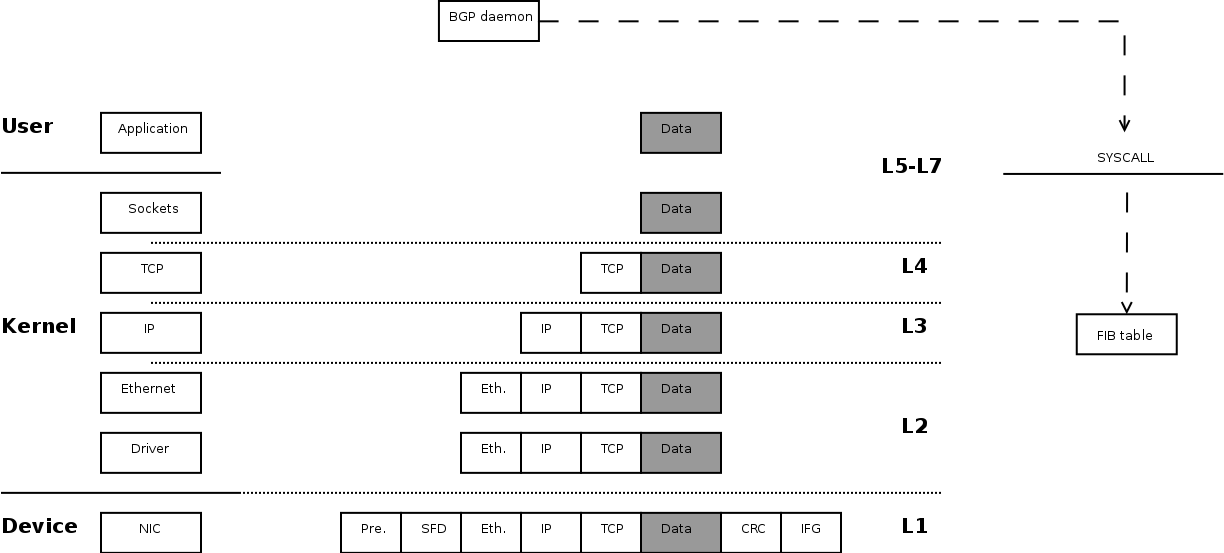
\includegraphics[width=10cm,keepaspectratio]{fig/layers.png}
		\end{figure}
\end{frame}

\begin{frame}{Reprezentace paketu - struct sk\_buff}
	\begin{figure}
		\centering
		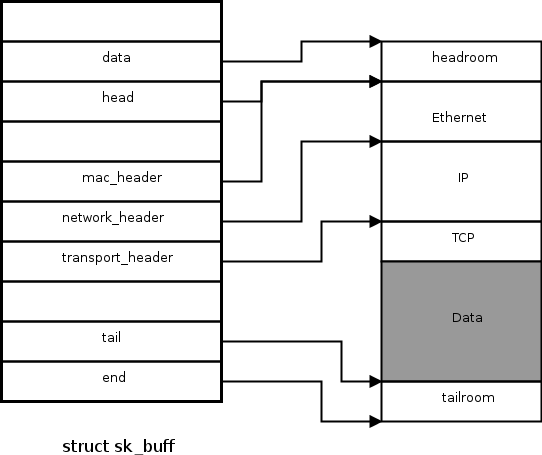
\includegraphics[width=6cm,keepaspectratio]{fig/skb.png}
	\end{figure}
\end{frame}

\begin{frame}{L3 - IPv4 stack}
	\begin{figure}
		\centering
		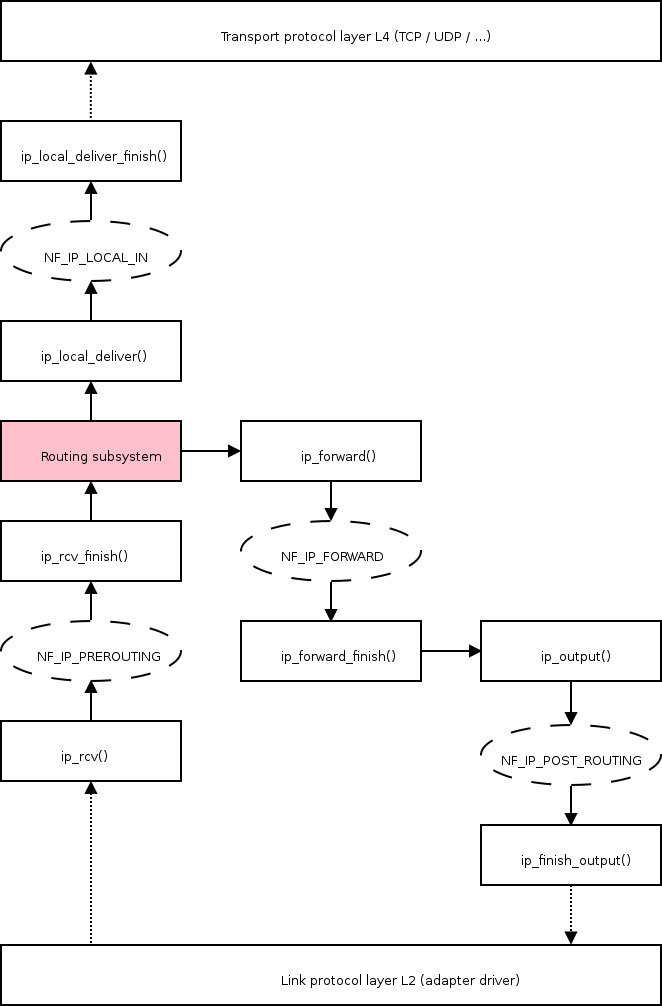
\includegraphics[width=6cm,height=6.5cm]{fig/kernel-layer3-flow.png}
	\end{figure}
\end{frame}

\begin{frame}{L2 - ovladače}
	\begin{itemize}
		\item Ovladač implementuje rozhraní {\href{http://lxr.free-electrons.com/source/include/linux/netdevice.h?v=4.0\#L1499}{struct net\_device}}
		\item Inicializace - alokace bufferů pro přenos paketů
		\item {\href{http://lxr.free-electrons.com/source/drivers/net/ethernet/intel/e1000e/netdev.c?v=4.0\#L7019}{register\_netdev(struct net\_device *)}}
		\item DMA přenosy do bufferu
		\item Obsluhuje IRQ
	\end{itemize}
\end{frame}

\begin{frame}{Původní zpracování paketů v Linuxu 2.4}
	\begin{itemize}
		\item DMA přenos do RX ring bufferu
		\item Přerušení IRQ - rutina provede nejnutnější práci
		\begin{itemize}
			\item Inicializace sk\_buff
			\item Aktualizace statistik
			\item Přidání do fronty CPU backlog - {\href{http://lxr.free-electrons.com/source/drivers/net/ethernet/3com/3c509.c?v=4.0\#L955}{netif\_rx(struct sk\_buff *)}}
			\item Naplánování NET\_RX\_SOFTIRQ
		\end{itemize}
		\item Zpracování paketu v softirq
	\end{itemize}
\end{frame}

\begin{frame}{Původní zpracování paketů - L2}
	\centering
	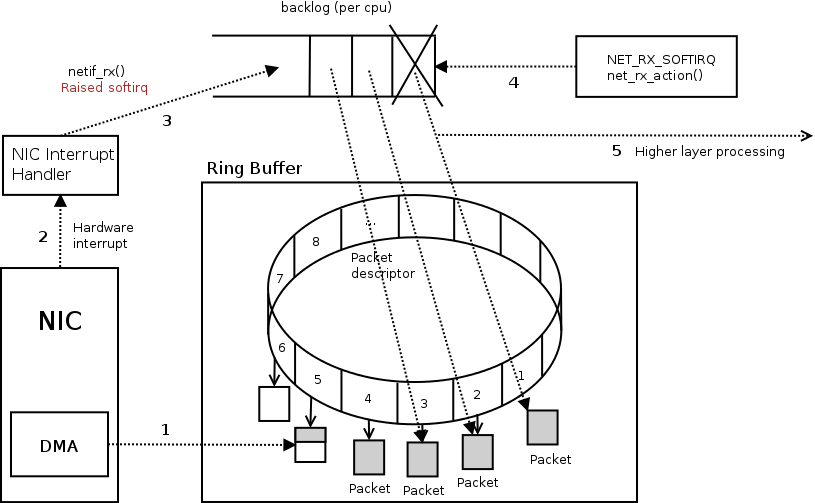
\includegraphics[width=9cm,keepaspectratio]{fig/non-napi.png}
	\\
	\begin{itemize}
		\item {\url{http://www.tldp.org/HOWTO/KernelAnalysis-HOWTO-8.html}}
	\end{itemize}
\end{frame}

\begin{frame}{Původní zpracování paketů - L3}
	\centering
	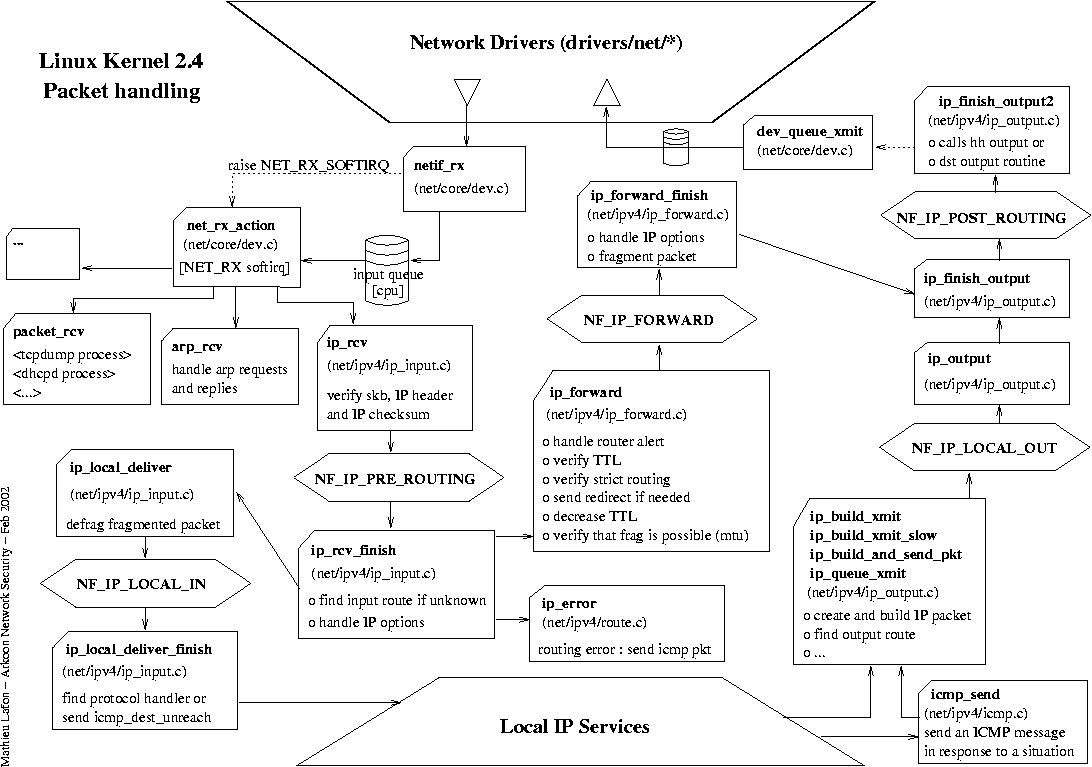
\includegraphics[width=10cm,keepaspectratio]{fig/kernel_24.png}
\end{frame}

\begin{frame}{100Mbit nestíháme - Linux 2.6 New API (NAPI)}
	\begin{itemize}
		\item 100Mbit - až 148~kpps
		\item Interrupt mitigation / coalescence
		\item První paket způsobí přeřušení
		\item Další pakety kernel vyzvedává ze síťové karty v rámci NET\_RX\_SOFTIRQ
		\item Nutné úpravy ovladače - struct net\_device$\rightarrow$poll()
		\item Karta musí mít možnost vypnout přerušení
		\item {\url{https://code.google.com/p/ldd3/source/browse/trunk/snull/snull.c}}
	\end{itemize}
\end{frame}

\begin{frame}{NAPI workflow}
	\centering
	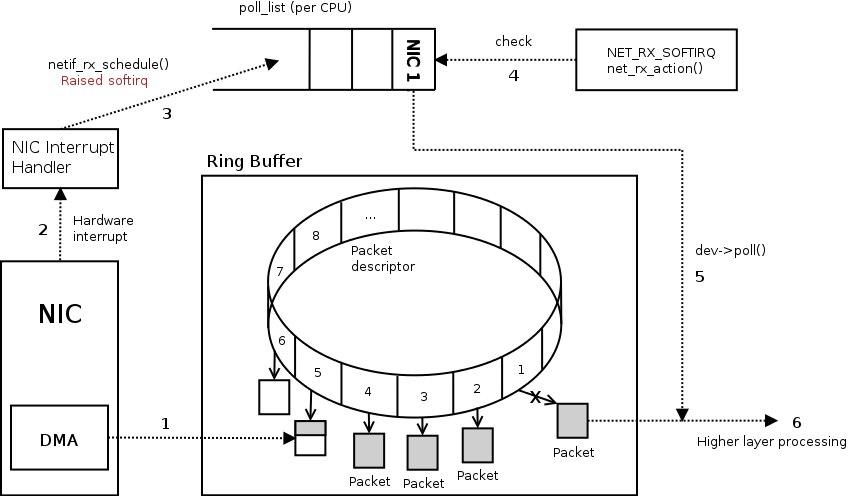
\includegraphics[width=10cm,keepaspectratio]{fig/napi-workflow.png}
\end{frame}

\begin{frame}{Zachraňujeme odezvu}
	\begin{itemize}
		\item Low Latency Sockets - setsockopt(SO\_BUSY\_POLL) - od Linuxu 3.11
		\item Řízení přerušení - ethtool -{}-show-coalesce eth0
	\end{itemize}
	\centering
	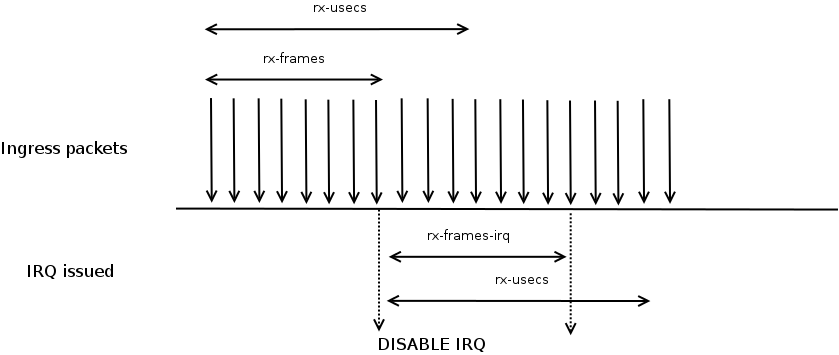
\includegraphics[width=9.5cm,keepaspectratio]{fig/irq-napi.png}
\end{frame}

%%%%%%%%%%%%%%%%%%%%%%%%%%%%%%%%%%%%%%%%%%%%%%%%%%%%%%%%%%%%%%%%%%%%%%%%
%%% HARDWARE %%%
%%%%%%%%%%%%%%%%%%%%%%%%%%%%%%%%%%%%%%%%%%%%%%%%%%%%%%%%%%%%%%%%%%%%%%%%

\begin{frame}{HARDWARE}
		\begin{figure}
			\centering
			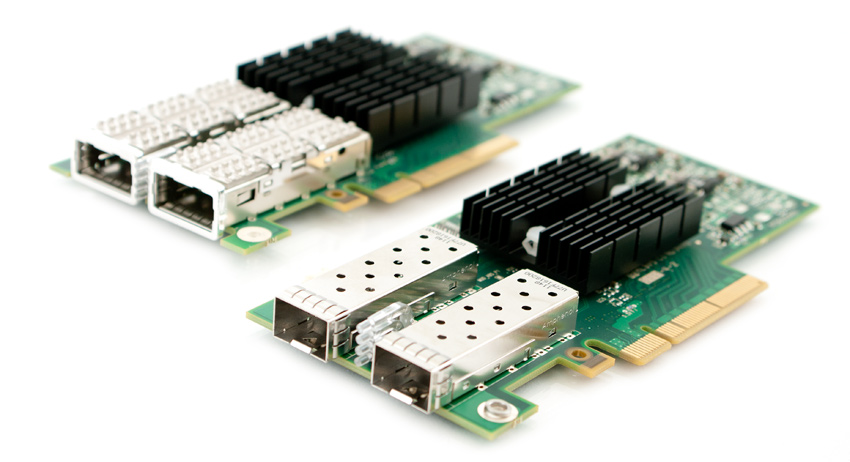
\includegraphics[width=8cm,keepaspectratio]{fig/nic.jpg}
		\end{figure}
\end{frame}

\begin{frame}{Offload mechanismy}
	\begin{itemize}
		\item Kontrolní součty
		\item Fragmentace IP
		\item Segmentace TCP
		\item Scatter-Gather - DMA přenos z více míst
		\item TCP Offload Engine - ACK, otevírání a uzavírání spojení - odmítnuto - rozbíjí Netfilter, Traffic Control
	\end{itemize}
\end{frame}

\begin{frame}{Generic Receive Offload - varianta bez GRO}
	\centering
	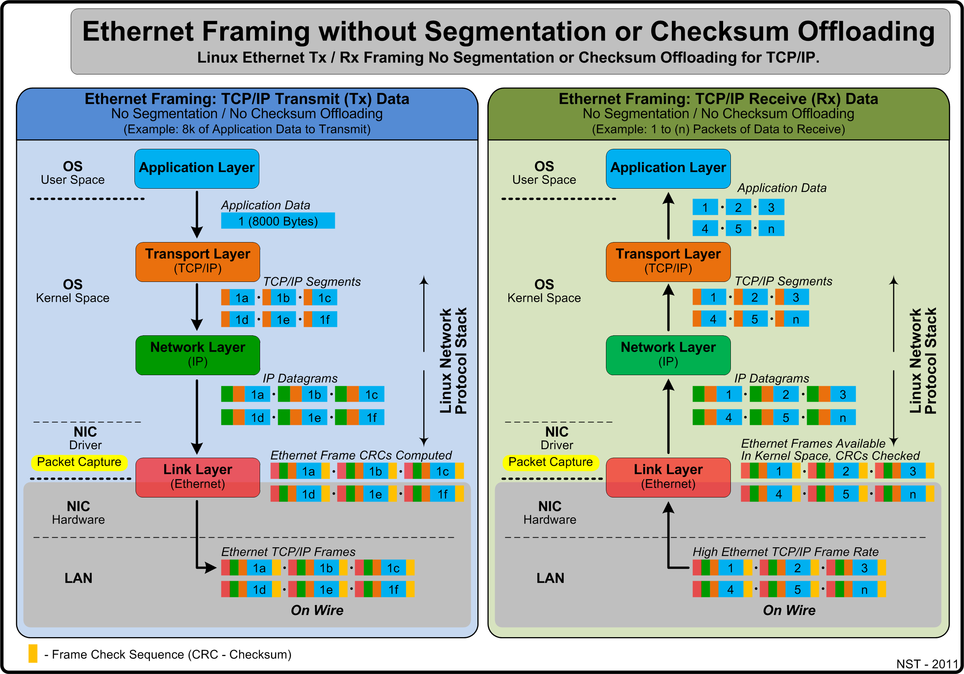
\includegraphics[width=10cm,keepaspectratio]{fig/no_segmentation_offloading.png}
\end{frame}

\begin{frame}{Generic Receive Offload - varianta s GRO}
	\centering
	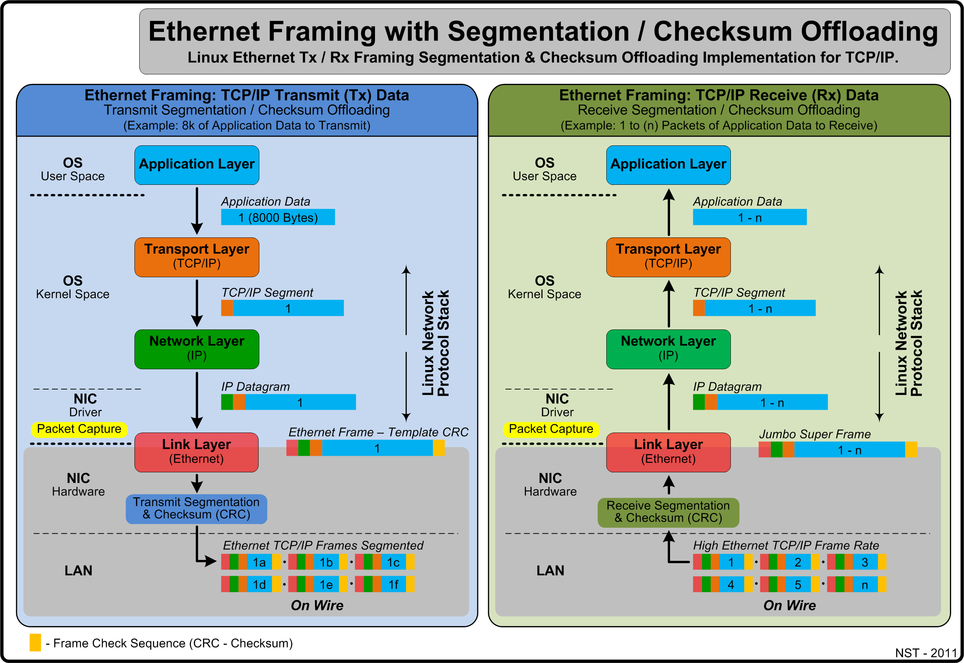
\includegraphics[width=10cm,keepaspectratio]{fig/segmentation_offloading.png}
\end{frame}

\begin{frame}[fragile]{Konfigurace Offload mechanismů}
	Zobrazení
	\begin{lstlisting}
		ethtool --show-offload eth0
	\end{lstlisting}
	Nastavení
	\begin{lstlisting}
		ethtool --offload eth0 rx on
	\end{lstlisting}
	Ovladač implementuje rozhraní struct ethtool\_ops
\end{frame}


\begin{frame}{Vícejádrové CPU - škálování - Linux 2.6.35}
	\begin{itemize}
		\item Škálování založeno různých síťových tocích - Hash nad hlavičkami
		\item Každé CPU může zpracovávat jiné toky
		\item Receive Packet Steering (RPS) - určení CPU softwarem
		\item Receive Side Steering (RSS) - určení CPU síťovou kartou pomocí přerušení (MSI-X)
		\item Vícefrontové síťové karty - Multiqueue NIC
	\end{itemize}
\end{frame}

\begin{frame}{Multiqueue NIC}
	\centering
	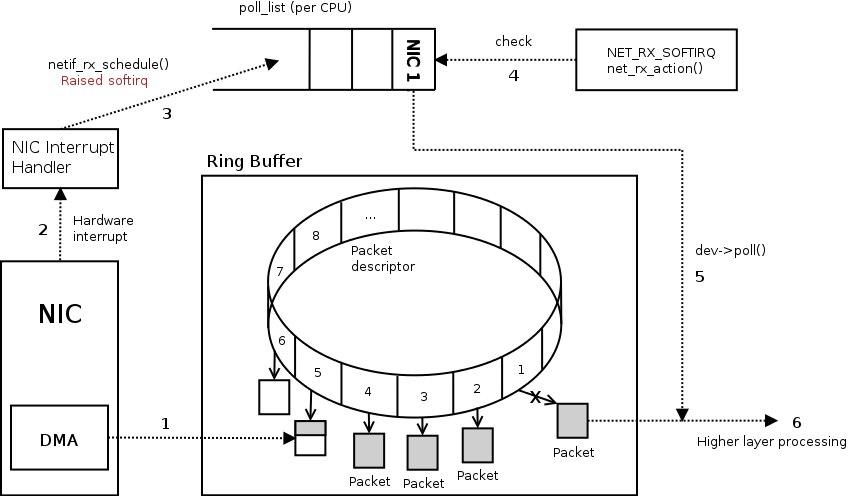
\includegraphics[width=3cm,keepaspectratio]{fig/napi-workflow.png} \\
	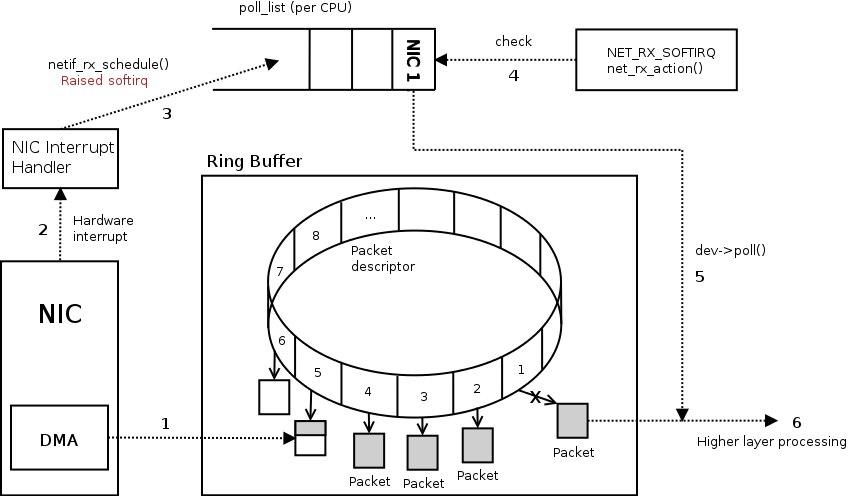
\includegraphics[width=3cm,keepaspectratio]{fig/napi-workflow.png} \\
	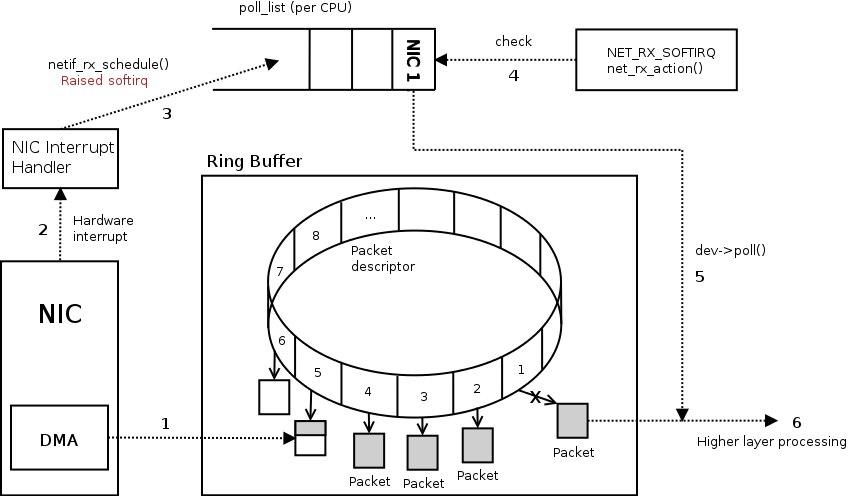
\includegraphics[width=3cm,keepaspectratio]{fig/napi-workflow.png} \\
	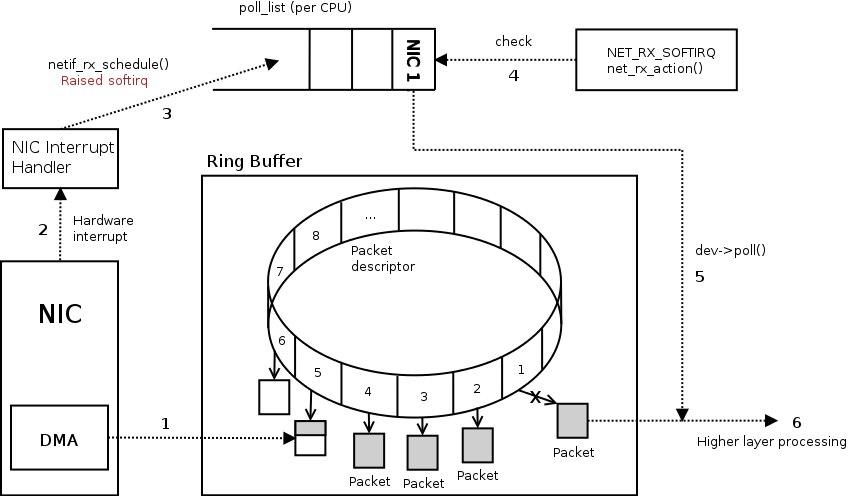
\includegraphics[width=3cm,keepaspectratio]{fig/napi-workflow.png} \\
\end{frame}

\begin{frame}{Architektura paralelního systému}
		\begin{figure}
			\centering
			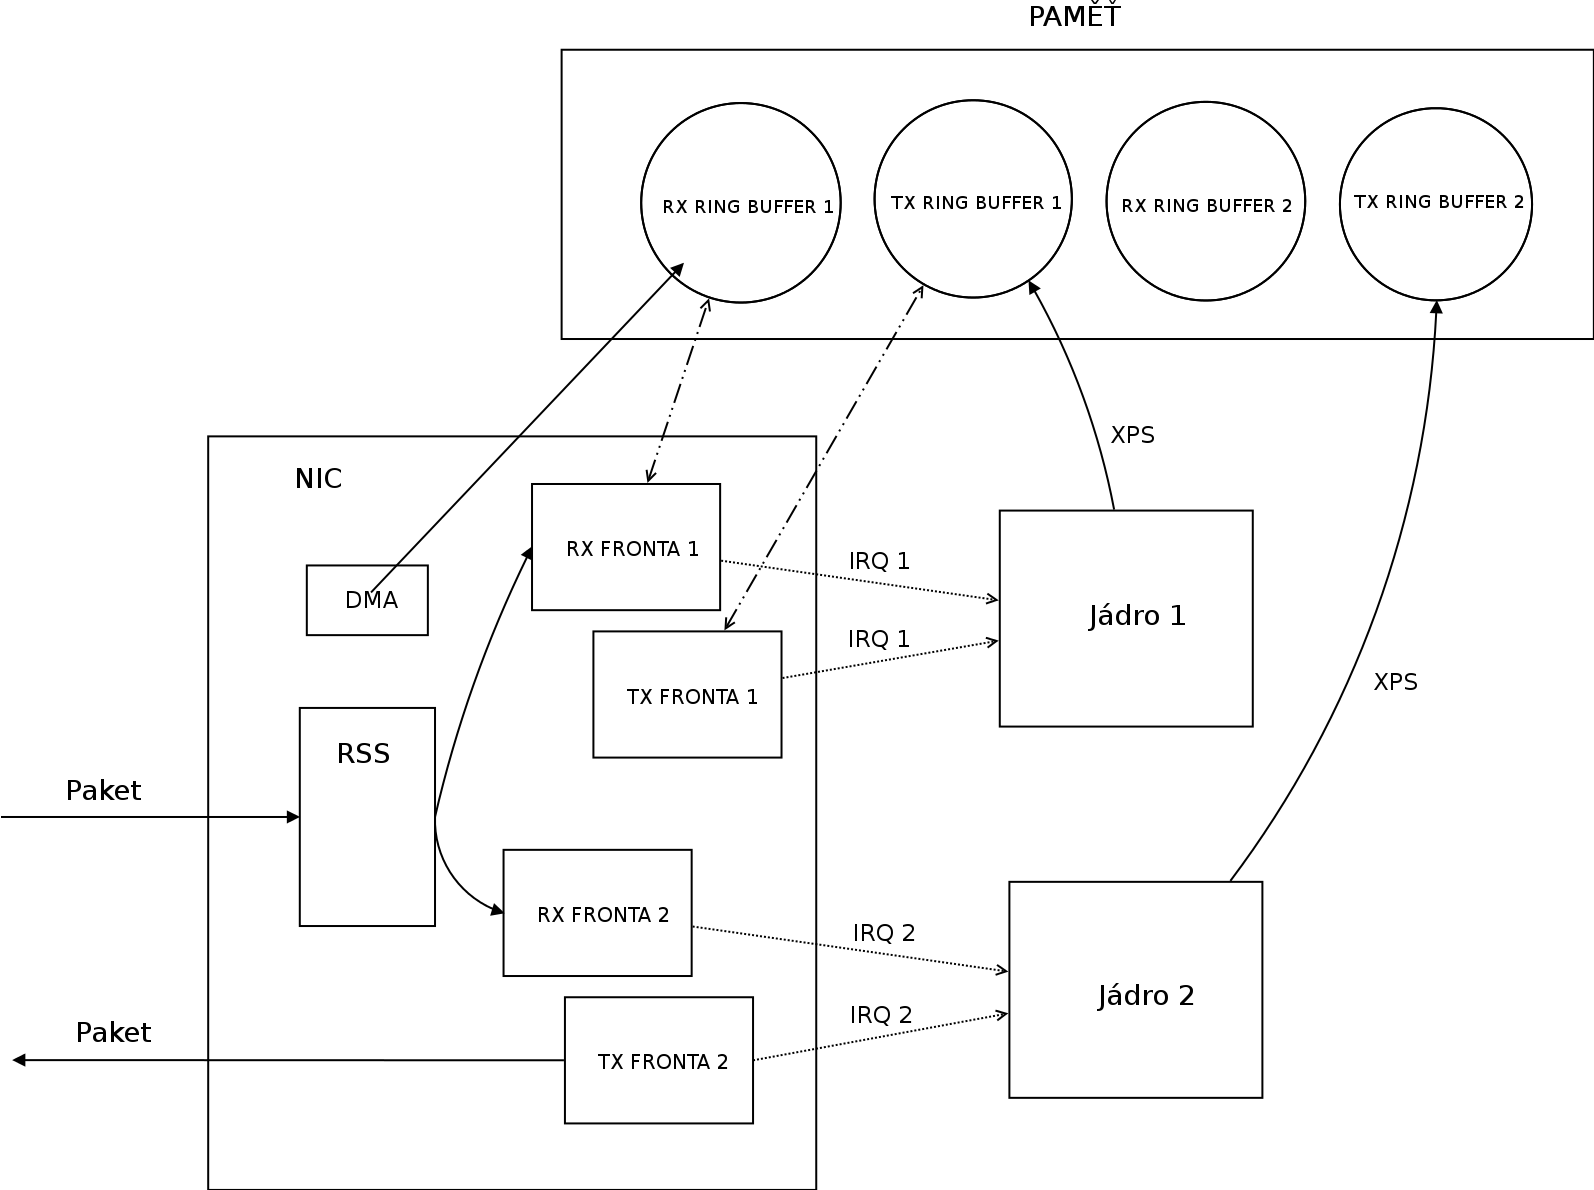
\includegraphics[width=8.75cm,keepaspectratio]{fig/arch.png}
		\end{figure}
\end{frame}

\begin{frame}{Receive Side Scaling}
	\begin{itemize}
		\item 32-bit Toeplitz hash nad IPs, protocol, ports, RSS Hash key
		\item Výsledek použit jako index do Indirection table
		\item Indirection table určí cílovou RX frontu \\
		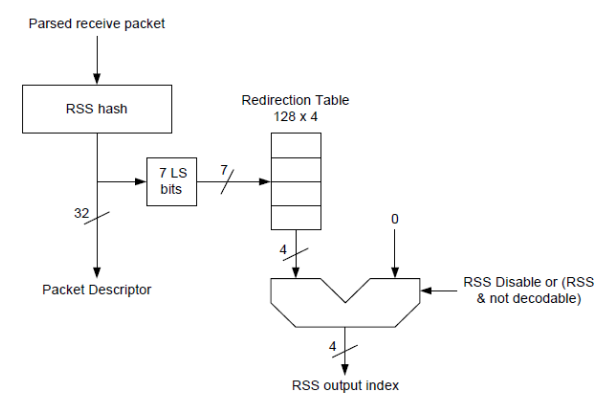
\includegraphics[width=8.5cm,keepaspectratio]{fig/rss.png}
	\end{itemize}
\end{frame}

\begin{frame}[fragile]{Konfigurace RSS}
	Nastavení počtu front
		\begin{lstlisting}
		ethtool --show-channels eth0
		ethtool --set-channels eth0 rx 4
		\end{lstlisting}
	Indirection table
		\begin{lstlisting}
		ethtool --show-rxfh-indir enp129s0
		\end{lstlisting}
	Mapování pomocí IRQ affinity
		\begin{lstlisting}
		cat /proc/interrupts
		echo "0-1,4" > /proc/irq/32/smp_affinity_list
		echo "013" > /proc/irq/32/smp_affinity
		\end{lstlisting}
	Nastavení RSS Hash key - symetrického
		\begin{lstlisting}
		ethtool --set-rxfh-indir enp129s0 hkey
		\end{lstlisting}
\end{frame}

\begin{frame}[fragile]{Accelerated Receive Flow Steering}
	Doručení paketu CPU na kterém běží cílová aplikace
		\begin{lstlisting}
		ethtool --show-offloads eth0 | grep ntuple
		ntuple-filters: on

		ethtool --config-nfc eth0 flow-type tcp4 src-ip
			10.0.0.1 dst-ip 10.0.0.2 src-port 10000
			dst-port 10001 action 6

		Added rule with ID 2045

		ethtool --show-nfc eth0
		\end{lstlisting}
\end{frame}


\begin{frame}[fragile]{Transmit Packet Steering (XPS) - kernel 2.6.38}
	Určíme které procesory mohou využít danou TX frontu
	\begin{lstlisting}
		/sys/class/net/eth0/queues/tx-0/xps_cpus
	\end{lstlisting}

	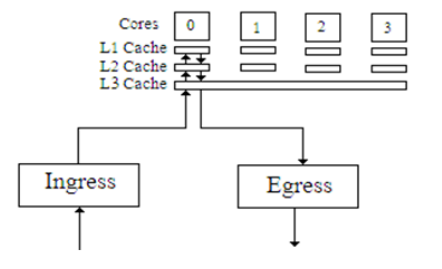
\includegraphics[width=5cm,keepaspectratio]{fig/irq-cache.png}
	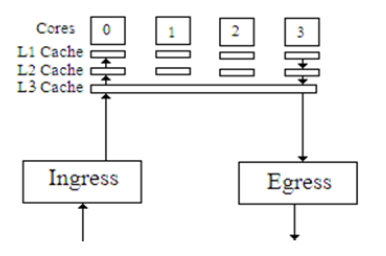
\includegraphics[width=5cm,keepaspectratio]{fig/irq-spread.png}
\end{frame}

\begin{frame}{Odesílání xmit\_more - kernel 3.19}
	Připravíme pakety do TX ring bufferu, ale neodesíláme je
	\begin{itemize}
		\item Paket (sk\_buff - obsahuje příznak xmit\_more)
		\item Paket (sk\_buff - obsahuje příznak xmit\_more)
		\item ...
		\item Paket (sk\_buff - neobsahuje xmit\_more) - DMA transfer, odeslání
	\end{itemize}
	pktgen zvládá generovat 14.88~Mpps na 1 CPU
\end{frame}

%%%%%%%%%%%%%%%%%%%%%%%%%%%%%%%%%%%%%%%%%%%%%%%%%%%%%%%%%%%%%%%%%%%%%%%%
%%% BENCHMARK %%%
%%%%%%%%%%%%%%%%%%%%%%%%%%%%%%%%%%%%%%%%%%%%%%%%%%%%%%%%%%%%%%%%%%%%%%%%

\begin{frame}{BENCHMARK}
		\begin{figure}
			\centering
			
\includegraphics[width=7cm,keepaspectratio]{fig/bench.png}
		\end{figure}
\end{frame}

\begin{frame}{10 a 40~GbE}
	\begin{itemize}
		\item 10~GbE - až 14.88~Mpps
		\item 40~GbE - až 59.5~Mpps (3.26~Mpps při payload 1518~B)
		\item Frame rates -  \\
		307.6 / 16.8~ns (51 cyklů na 3~GHz CPU)
		\item Propustnost - 4.6~GB/s (PCIe 2.0 x8 4~GB/s, PCIe 3.0 x8 7.9~GB/s)
		\item 40GBASE-T s dosahem 30m
	\end{itemize}
\end{frame}

\begin{frame}{SW nastavení pro L1-L3}
	\begin{itemize}
		\item RSS a smp\_affinity
		\item XPS
		\item Offloads
		\item Netfilter
		\item Zpracování ARP/ND
		\item SELinux
		\item Reverse Path filter
		\item Pakety pro lokální aplikace (BGPd) - na separátním CPU (kartě / frontě)
	\end{itemize}
\end{frame}

\begin{frame}{Hardware}
	\begin{itemize}
		\item NIC - RSS, Offloads
		\item Počet jader
		\item Velikost L1,L2,L3 cache
		\item Intel Xeon - Direct Cache Access (DDIO)
		\item Hyper-Threading
	\end{itemize}
\end{frame}

\begin{frame}{Vliv nastavení}
	\begin{figure}
		\centering
		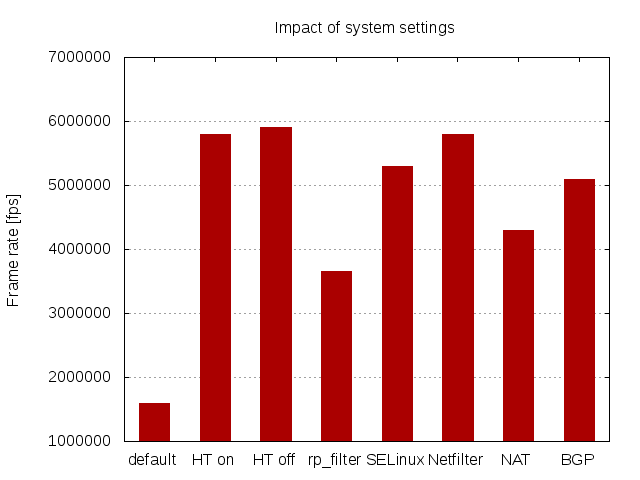
\includegraphics[width=8cm,keepaspectratio]{fig/settings.png}
	\end{figure}
\end{frame}

\begin{frame}{Frames per second}
	\begin{figure}
		\centering
		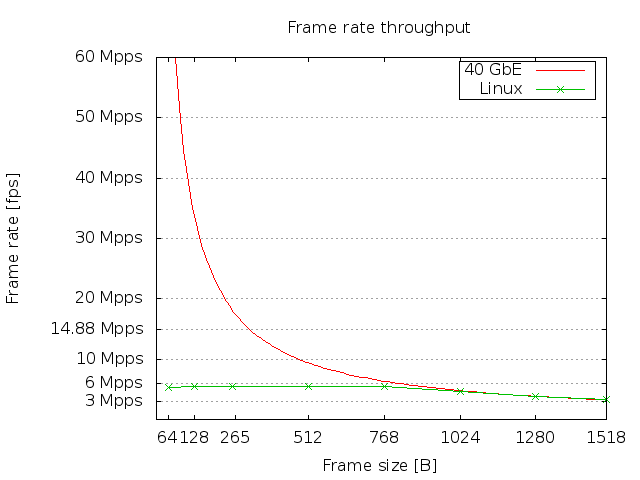
\includegraphics[width=8cm,keepaspectratio]{fig/frames.png}
	\end{figure}
\end{frame}

\begin{frame}{Propustnost v gigabitech}
	\centering
	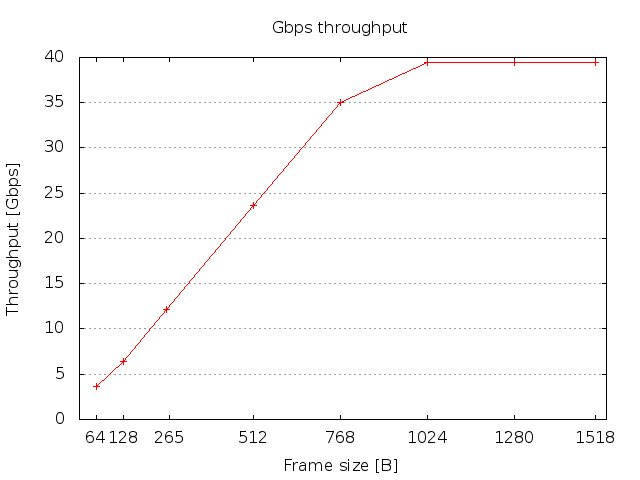
\includegraphics[width=8cm,keepaspectratio]{fig/gigabits.png}
\end{frame}

\begin{frame}{Velikost rámců v AMS-IX}
	\begin{figure}
		\centering
		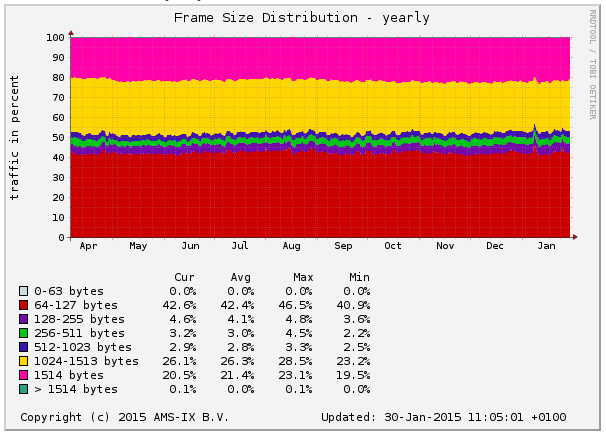
\includegraphics[width=8cm,keepaspectratio]{fig/amsix.png}
	\end{figure}
\end{frame}

\begin{frame}{Výkonnost podle velikosti rámců}
	\begin{tabular}{ | l | l | l | l |}
	\hline
	Frame size & \% of 40Gb link & bandwidth & frame rate \\
	\hline
	64     &  8.99\% &  3.60~Gb/s & 5~350~000 \\
	594    & 68.15\% & 27.26~Gb/s & 5~550~000 \\
	1518   & 99.60\% & 39.40~Gb/s & 3~202~210 \\
	AMS-IX & 88.25\% & 35.30~Gb/s & 5~800~000 \\
	\hline
	\end{tabular}
\end{frame}

\begin{frame}[fragile]{Profilování Linuxu}
	1 jádro
	\begin{lstlisting}[basicstyle=\ttfamily]
	11.42%  [kernel]  [k] fib_table_lookup
	 9.62%  [kernel]  [k] _raw_spin_lock
	 6.65%  [kernel]  [k] mlx4_en_xmit
	 4.84%  [kernel]  [k] memcpy
	 4.03%  [kernel]  [k] mlx4_en_complete_rx_desc
	\end{lstlisting}
	
	RSS na 8 jádrech
	\begin{lstlisting}[basicstyle=\ttfamily]
	12.07%  [kernel]  [k] _raw_spin_lock
	 8.68%  [kernel]  [k] fib_table_lookup
	 5.01%  [kernel]  [k] mlx4_en_xmit
	 4.63%  [kernel]  [k] mlx4_en_process_rx_cq
	 3.49%  [kernel]  [k] memcpy
	\end{lstlisting}
\end{frame}
	
	\begin{frame}{Ostatní systémy}
	\begin{itemize}
		\item FreeBSD - \url{http://bsdrp.net/documentation/technical_docs/performance}
		\item Cisco HW - \url{http://www.cisco.com/web/partners/downloads/765/tools/quickreference/routerperformance.pdf}
	\end{itemize}
\end{frame}

\begin{frame}
	Odkazy: \\
	{\url{https://wiki.freebsd.org/201305DevSummit/NetworkReceivePerformance/ComparingMutiqueueSupportLinuxvsFreeBSD}}
	{\url{http://www.intel.com/content/dam/www/public/us/en/documents/white-papers/multi-core-processor-based-linux-paper.pdf}}
\end{frame}

\end{document}
